\subsubsection{Instructions}
This guide describes the steps required to solder and assemble HestiaPi Touch ONE
from parts.  Assembly with the case and wall is not covered here.

\subsubsection{Video}
\href{https://www.youtube.com/watch?v=gRcRINqT31g}{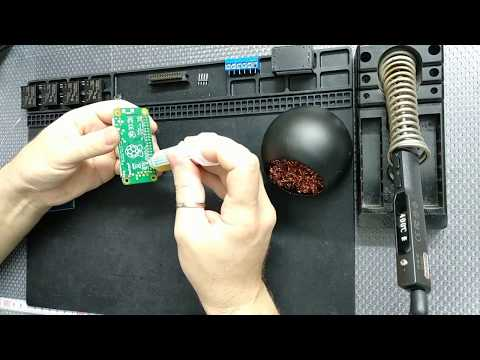
\includegraphics[width=5.0in]{img/hestiapi_one_soldering.jpg}}

\subsubsection{Hints and Tips}
The LCD needs to be connected before powering HestiaPi as it initialises on
boot only (otherwise it looks blank-white and touch events do not register) and
it may also cause a freeze or reboot due to power spike.

If you cannot control mains, that is having it off during all the time of
installation, our advise is to leave the SD card and LCD out, connect all
wires, partly (not fully) insert the SD and finish off case installation with
the LCD attached to the cover.

Once all is done, from outside of the case, push first the SD all the way in
(it does not lock-click in place) and then insert a non-metallic tool and press
the reset button from the right side. HestiaPi will boot and in about 10-15sec
the LCD will show some of the boot messages.
